
The one-dimensionnal hydro-sedimentary code \courlis is designed to simulate sediment transport in rivers and reservoirs where the flows can be considered as 1D. It is weakly coupled with the one-dimensionnal hydrodynamic software \mascaret. Both are part of the open-source system \telemacsystem (\texttt{www.opentelemac.org}).

\begin{figure}[htb!]
    \centering
    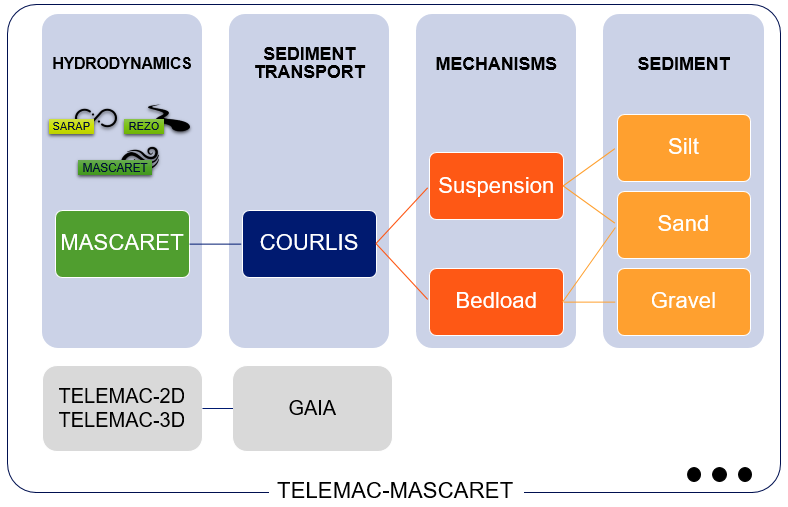
\includegraphics[width=\textwidth]{./graphics/telemac.png}
    \caption{\courlis within the \telemacsystem}
    \label{fig:telemac}
\end{figure}

The software supports steady and unsteady flow computations thanks to the three computational kernels of \mascaret :
\begin{itemize}
	\item SARAP : the steady flow kernel for subcritical, supercritical or mixed flow regimes (finite differences)
	\item REZO : the unsteady subcritical flow kernel (finite differences)
	\item MASCARET : the unsteady trans-critical flow kernel (finite volumes)
\end{itemize}
Complete description of those kernels can be found in the \mascaret guides. \mascaret computes surface elevations, discharge and velocities along the bief. These variables are then passed to the module \courlis to calculate sediment transport capacity and bed evolutions.  

Two options are available in \courlis to model sediment transport : 
\begin{itemize}
	\item Modelling suspended load : the sediment particles are transported by the flow and maintained (possibly temporary) in suspension above the bottom by the action of shear stress at bottom. 
	\item Modelling bedload : the sediment particles are transported in direct contact with the bottom or next to the bed without being affected by the fluid turbulence.
\end{itemize}
In physical systems, both mechanisms are generally observed but their mathematical representation are quite different. In \courlis suspended load is the solution of an advection-diffusion equation with erosion and deposition fluxes while bedload is estimated thanks to closure relantionships for sediment transport capacity and a continuity equation for the bed (Exner equation). 

\begin{figure}[htb!]
    \centering
    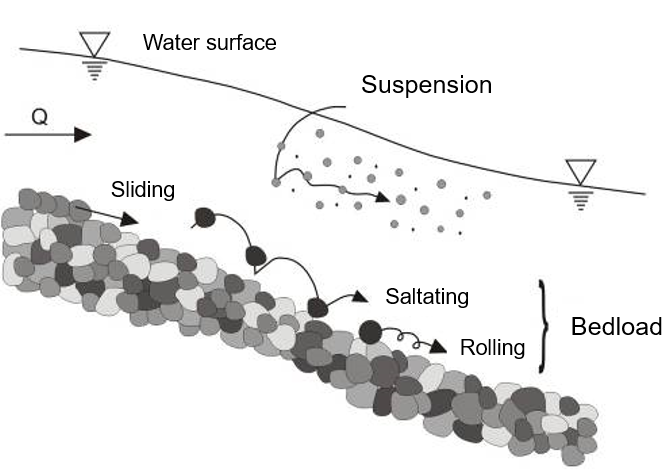
\includegraphics[width=.8\textwidth]{./graphics/transport_mechanisms.png}
    \caption{Sketch summarizing sediment transport mechanisms - saltation can be modeled with both bedload and suspended load modules (extracted from \cite{univ_lyon})}
    \label{fig:mechanisms}
\end{figure}

\Csuspension model both cohesive (fine particles such as silt or clay) or non-cohesive sediment (sand). 
\Cbedload is usually used to model gravel or coarse sand transport. 

\begin{figure}[htb!]
    \centering
    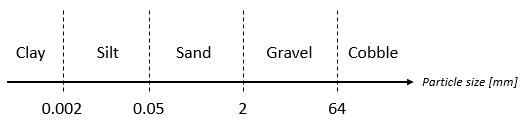
\includegraphics[width=0.8\textwidth]{./graphics/sediment_sizes.png}
    \caption{Canadian system soil classification also called SCCS classification (1987)}
    \label{fig:sediment_sizes}
\end{figure}





